%%% template.tex
%%%
%%% This LaTeX source document can be used as the basis for your technical
%%% paper or abstract. Intentionally stripped of annotation, the parameters
%%% and commands should be adjusted for your particular paper - title, 
%%% author, article DOI, etc.
%%% The accompanying ``template.annotated.tex'' provides copious annotation
%%% for the commands and parameters found in the source document. (The code
%%% is identical in ``template.tex'' and ``template.annotated.tex.'')

\documentclass[conference]{acmsiggraph}

\usepackage{authblk}

\TOGonlineid{45678}
\TOGvolume{0}
\TOGnumber{0}
\TOGarticleDOI{1111111.2222222}
\TOGprojectURL{}
\TOGvideoURL{}
\TOGdataURL{}
\TOGcodeURL{}



\title{A Greedy Heuristic using Redundancy for the Data Layout Problem}

\author[1]{Shan Jiang\thanks{sjiang1714@gmail.com}}
\author[1]{Zachary DeStefano\thanks{zdestefa@uci.edu}}
\author[1]{Gopi Meenakshisundaram\thanks{gopi.meenakshisundaram@gmail.com}}
\author[2]{Sung-Eui Yoon\thanks{toinsert}}
\pdfauthor{Zachary DeStefano,Shan Jiang,Gopi Meenakshisundaram,Sung-Eui Yoon}
\affil[1]{University of California, Irvine}
\affil[2]{KAIST}

\keywords{Data Layout Problem, Out-Of-Core Rendering, Cache Oblivious Mesh Layout}

\begin{document}

%% \teaser{
%%   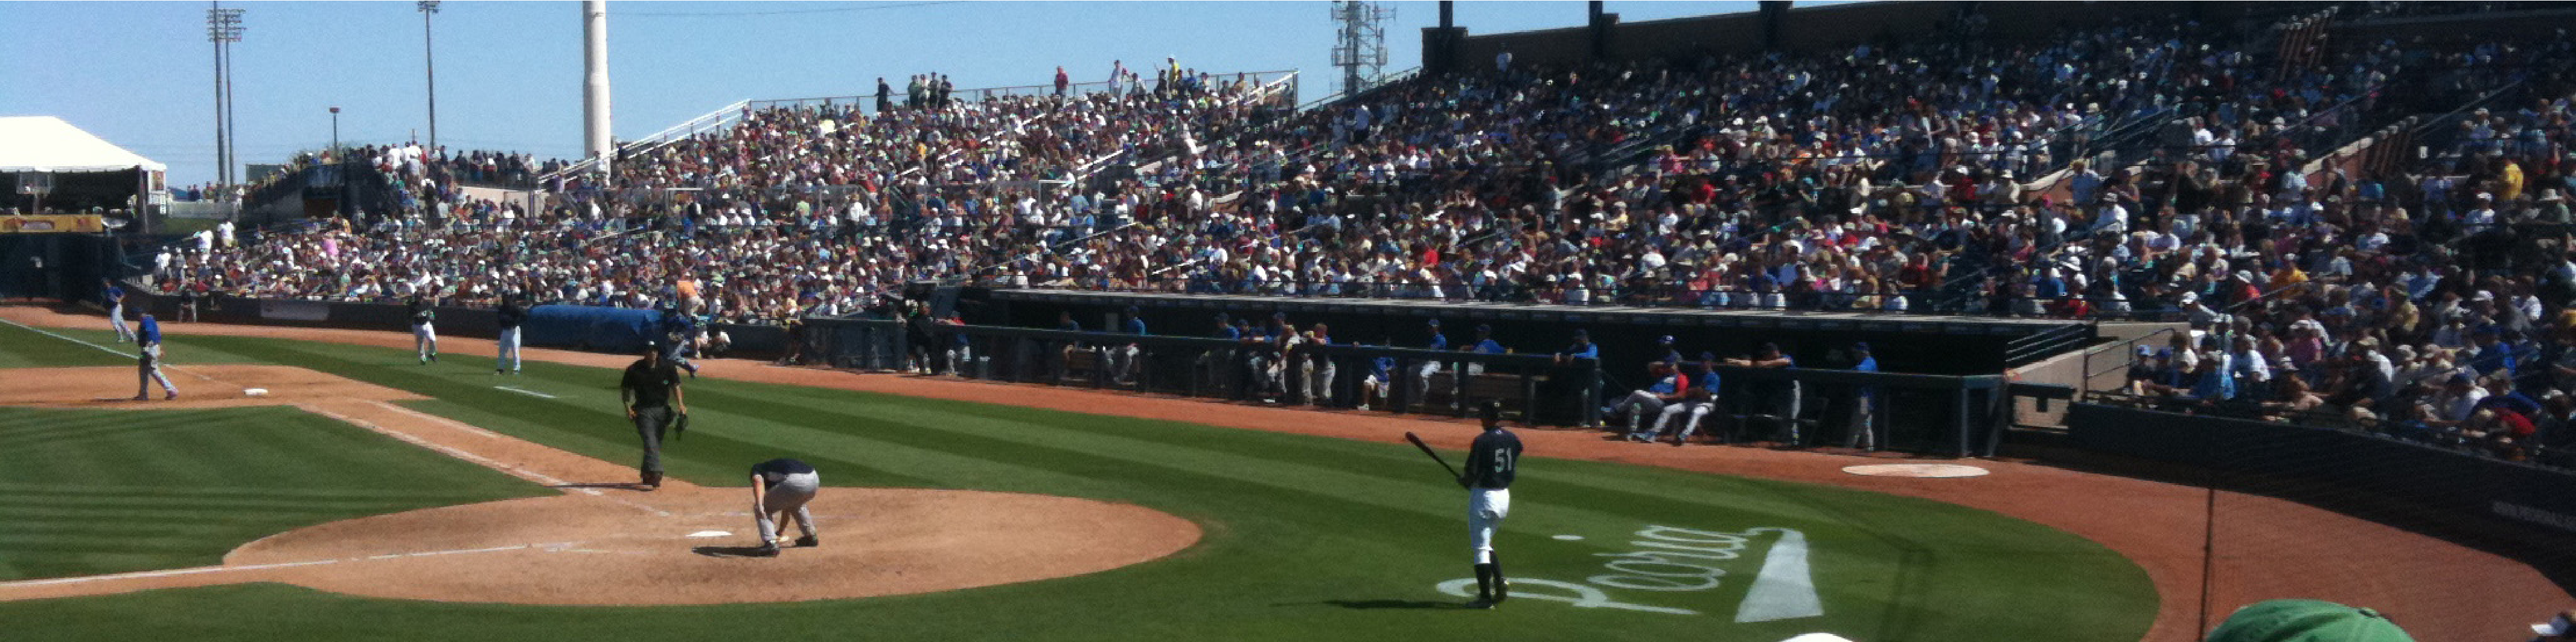
\includegraphics[height=1.5in]{images/sampleteaser}
%%   \caption{Spring Training 2009, Peoria, AZ.}
%% }

\maketitle

\begin{abstract}

In Computer Graphics, in order to compute an efficient cache oblivious mesh layout we must figure out the optimal method for laying out the data units. Finding a deterministic solution to the problem is NP-hard so various heuristics have been proposed. In this paper, we present a solution to the problem based on introducing redundancy to the layout. It will reduce seek time while using the least amount of redundancy possible. This will prove to be a better heuristic than existing ones proposed both analytically and experimentally. 

\end{abstract}

\begin{CRcatlist}
  \CRcat{I.3.6}{Computer Graphics}{Methodology and Techniques}{Graphics data structures and data types};
\end{CRcatlist}

\keywordlist

%% Use this only if you're preparing a technical paper to be published in the 
%% ACM 'Transactions on Graphics' journal.

\TOGlinkslist

%% Required for all content. 

\copyrightspace

\section{Introduction}

The Data Layout Problem can be formulated as follows. The input is a linear sequence of data units. Each of the data units is assigned at least one color and many of them have multiple colors assigned. The length of a color is the distance from its first data unit to its last data unit. The data units can be rearranged as desired. The output we would like is the sequence of data units that will minimize the total length of all the colors. \\
\\
In Yoon's paper \cite{cacheobliviouslayout}, the Data Layout Problem is described as well as the metric that is motivating the above definition. We noticed that access patterns described in the paper can be very general and there could easily be data units that are far apart in the sequence but need to be accessed together. This led us to realize that if we copy data units and move them closer to other ones that share the same access pattern then we could save a lot of seek time without adding much storage space. The rest of this paper is about the algorithm developed to optimize seek time while minimizing the redundancy required to accomplish that. 

\section{Related Work}

Massive model rendering has been a challenging field of research in computer graphics for decades. A large body of literature has been built on different aspects of solving this problem. Here we briefly discuss work in two main approaches in this topic, Out-Of-Core Rendering and Image-based Rendering. 

\subsection{Out-Of-Core Rendering}

Large-scale model rendering generally implies that the geometry data is so large that one must employ a secondary storage device during rendering. Thus, due to the nature of secondary storage devices and the architecture of modern computers, data fetching and data management for main memory can become performance bottlenecks during rendering. To remove or reduce these bottlenecks, research on out-of-core rendering aims at fetching, caching, and managing data in efficient ways. Coorea et al \cite{iwalk} introduced the iWalk system, in which octree-based spatialization is applied on geometry data, and this allowed only visible data to be retrieved from hard drives. Varadhan et al \cite{outofcore} also focused on isolating data required by each frame, but in a graph-based algorithm. A scene graph is generated in level of details and frame-to-frame visibility consistence. Parallel processing is also employed so that rendering the active part of the scene and fetching objects from the disk are done simultaneously. Sajadi et al \cite{pagebased} improved efficiency of out-of-core rendering by preprocessing the data set into a form of disk pages. The disk pages are self-contained data units with fixed size. This method avoids data management on the primitive level which reduces the time complexity by orders of magnitude. By utilizing a globally optimized data layout, caching can be further improved. Globally optimized data layout is an NP hard problem. Nevertheless, Yoon et al \cite{cacheobliviouslayout} provided a feasible method to try to compute it. Similar to other problems where an optimal permutation needs to be computed, they developed a hierarchical algorithm with a heuristic based on edge spans to get an approximated solution quickly.

\subsection{Image-Based Rendering}

Image-based rendering techniques reduce the geometry of a massive model to a view-independent mesh along with pre-rendered textures. The number of primitives to be rendered is much less than the original model. Therefore, both data transferring time and rendering time can be greatly saved. The major drawback of image-based rendering is the lack of geometry information. Zhang et al \cite{imagebasedrendering} presented a survey of image-based rendering techniques. These techniques involve sampling the space using a plenoptic function in the first stage and then rendering the continuous plenoptic function in the next stage. It is similar to the technique in signal processing of sampling a set of numbers and then using those samples to get the continuous function and reconstructing the continuous function. The paper goes into detail on various applications of these techniques. Li et al \cite{compressionimagebased} explored various compression methods for image-based rendering. Specifically, they explored the benefits of three compression algorithms. All three proved to be able to achieve real time rendering of large models and they vary in the complexity of the decoding and the compression ratio they are able to achieve. 

\subsection{Seek Time and Redundancy-based solutions}

In real time rendering, time spent on one frame can be roughly divided into data fetching time, online processing time, and rendering time. Data fetching time can be further decomposed into seek time and data transfer time. Sajadi et al \cite{ssdpaper} explored the reasons for the performance advantage of Solid-State Drives (SSD) over Hard-Disk Drives (HDD). The result shows clearly constant seek time of SSDs is the major reason that fetching data on SSDs is generally faster and more consistent than HDDs. Jiang et al \cite{singleseeklayout} minimized disk seeks to one or less for each frame by storing multiple copies of same data at different locations of secondary storage devices. These extra copies will be referred to as redundancy. The paper successfully showed that limited seeks lead to improvement of performance. However, to keep number of seeks being one or less, a large amount of redundancy is necessary, which is not practical for many applications. Jiang et al \cite{optimizingredundancy} generalized this approach by relaxing the number of seeks to a small threshold. This threshold is determined by time budget of each frame. In this way, the number of seeks required is relaxed to minimize amount of redundancy. This optimization is done through integer linear programming. This approach ended up reducing the amount of redundancy significantly. The algorithm however does not take data layout into account and is thus not an optimal solution.

\section{Exposition}

Lorem ipsum dolor sit amet, consectetur adipisicing elit, sed do
eiusmod tempor incididunt ut labore et dolore magna aliqua. Ut enim ad
minim veniam, quis nostrud exercitation ullamco laboris nisi ut
aliquip ex ea commodo consequat. Duis aute irure dolor in
reprehenderit in voluptate velit esse cillum dolore eu fugiat nulla
pariatur. Excepteur sint occaecat cupidatat non proident, sunt in
culpa qui officia deserunt mollit anim id est laborum.

Lorem ipsum dolor sit amet, consectetur adipisicing elit, sed do
eiusmod tempor incididunt ut labore et dolore magna aliqua. Ut enim ad
minim veniam, quis nostrud exercitation ullamco laboris nisi ut
aliquip ex ea commodo consequat. Duis aute irure dolor in
reprehenderit in voluptate velit esse cillum dolore eu fugiat nulla
pariatur. Excepteur sint occaecat cupidatat non proident, sunt in
culpa qui officia deserunt mollit anim id est laborum.
%\begin{figure}[ht]
%  \centering
%  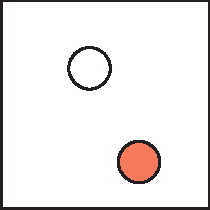
\includegraphics[width=1.5in]{images/samplefigure}
%  \caption{Sample illustration.}
%\end{figure}
Lorem ipsum dolor sit amet, consectetur adipisicing elit, sed do
eiusmod tempor incididunt ut labore et dolore magna aliqua. Ut enim ad
minim veniam, quis nostrud exercitation ullamco laboris nisi ut
aliquip ex ea commodo consequat. Duis aute irure dolor in
reprehenderit in voluptate velit esse cillum dolore eu fugiat nulla
pariatur. Excepteur sint occaecat cupidatat non proident, sunt in
culpa qui officia deserunt mollit anim id est laborum.

Lorem ipsum dolor sit amet, consectetur adipisicing elit, sed do
eiusmod tempor incididunt ut labore et dolore magna aliqua. Ut enim ad
minim veniam, quis nostrud exercitation ullamco laboris nisi ut
aliquip ex ea commodo consequat. Duis aute irure dolor in
reprehenderit in voluptate velit esse cillum dolore eu fugiat nulla
pariatur. Excepteur sint occaecat cupidatat non proident, sunt in
culpa qui officia deserunt mollit anim id est laborum.

Lorem ipsum dolor sit amet, consectetur adipisicing elit, sed do
eiusmod tempor incididunt ut labore et dolore magna aliqua. Ut enim ad
minim veniam, quis nostrud exercitation ullamco laboris nisi ut
aliquip ex ea commodo consequat. Duis aute irure dolor in
reprehenderit in voluptate velit esse cillum dolore eu fugiat nulla
pariatur. Excepteur sint occaecat cupidatat non proident, sunt in
culpa qui officia deserunt mollit anim id est laborum.

\section{Exposition}

Lorem ipsum dolor sit amet, consectetur adipisicing elit, sed do
eiusmod tempor incididunt ut labore et dolore magna aliqua. Ut enim ad
minim veniam, quis nostrud exercitation ullamco laboris nisi ut
aliquip ex ea commodo consequat. Duis aute irure dolor in
reprehenderit in voluptate velit esse cillum dolore eu fugiat nulla
pariatur. Excepteur sint occaecat cupidatat non proident, sunt in
culpa qui officia deserunt mollit anim id est laborum.

Lorem ipsum dolor sit amet, consectetur adipisicing elit, sed do
eiusmod tempor incididunt ut labore et dolore magna aliqua. Ut enim ad
minim veniam, quis nostrud exercitation ullamco laboris nisi ut
aliquip ex ea commodo consequat. Duis aute irure dolor in
reprehenderit in voluptate velit esse cillum dolore eu fugiat nulla
pariatur. Excepteur sint occaecat cupidatat non proident, sunt in
culpa qui officia deserunt mollit anim id est laborum.

Lorem ipsum dolor sit amet, consectetur adipisicing elit, sed do
eiusmod tempor incididunt ut labore et dolore magna aliqua. Ut enim ad
minim veniam, quis nostrud exercitation ullamco laboris nisi ut
aliquip ex ea commodo consequat. Duis aute irure dolor in
reprehenderit in voluptate velit esse cillum dolore eu fugiat nulla
pariatur. Excepteur sint occaecat cupidatat non proident, sunt in
culpa qui officia deserunt mollit anim id est laborum.

Lorem ipsum dolor sit amet, consectetur adipisicing elit, sed do
eiusmod tempor incididunt ut labore et dolore magna aliqua. Ut enim ad
minim veniam, quis nostrud exercitation ullamco laboris nisi ut
aliquip ex ea commodo consequat. Duis aute irure dolor in
reprehenderit in voluptate velit esse cillum dolore eu fugiat nulla
pariatur. Excepteur sint occaecat cupidatat non proident, sunt in
culpa qui officia deserunt mollit anim id est laborum.

Lorem ipsum dolor sit amet, consectetur adipisicing elit, sed do
eiusmod tempor incididunt ut labore et dolore magna aliqua. Ut enim ad
minim veniam, quis nostrud exercitation ullamco laboris nisi ut
aliquip ex ea commodo consequat. Duis aute irure dolor in
reprehenderit in voluptate velit esse cillum dolore eu fugiat nulla
pariatur. Excepteur sint occaecat cupidatat non proident, sunt in
culpa qui officia deserunt mollit anim id est laborum.

\section{Conclusion}

Lorem ipsum dolor sit amet, consectetur adipisicing elit, sed do
eiusmod tempor incididunt ut labore et dolore magna aliqua. Ut enim ad
minim veniam, quis nostrud exercitation ullamco laboris nisi ut
aliquip ex ea commodo consequat. Duis aute irure dolor in
reprehenderit in voluptate velit esse cillum dolore eu fugiat nulla
pariatur. Excepteur sint occaecat cupidatat non proident, sunt in
culpa qui officia deserunt mollit anim id est laborum.

\section*{Acknowledgements}

To Robert, for all the bagels.

\bibliographystyle{acmsiggraph}
\bibliography{finalPaperRefs}
\end{document}
